\chapter{Introdução à Álgebra Linear}
\label{cap:introdução}

Estas notas de aula destinam-se aos estudantes da FGV-EMAp que estão cursando a disciplina "Álgebra Linear", com o Prof. Guilherme Tegoni Goedert. Álgebra Linear é uma disciplina considerada difícil pela maioria dos estudantes. É a primeira vez em que as ideias atingem um nível muito alto de abstração. Ao mesmo tempo, porém, e justamente por isso, é uma das áreas mais fascinantes e importantes da Matemática.

De fato, algumas das suas aplicações são:

\begin{itemize}
	\item Resolução de sistemas de equações diferenciais ordinárias;
	\item Modelagem de circuitos elétricos;
	\item Modelos epidemiológicos;
	\item Manipulação de imagens e de vídeos;
	\item Aprendizado de máquinas.
\end{itemize}

Através destas notas de aula, eu pretendo ajudar os estudantes a entenderem todas as ferramentas que a Álgebra Linear desenvolve e utiliza, fornecendo uma sólida base teórica, e, de igual modo, ilustrando com algumas de suas aplicações.

\section{Representação Geométrica de Sistemas Lineares}

\textbf{Importante:} este capítulo é baseado em \cite{slide1doyuri}

Em Álgebra Linear, nós estamos interessados em um problema principal, que é a base de todo o ferramental teórico que será desenvolvido: "Como podemos resolver um sistema linear de $m$ equações e $n$ variáveis? Quando é possível fazer isto?".

Para responder a esta pergunta, é necessário primeiramente definir o que é um sistema linear:

\begin{Definition}[Sistema linear]
	Um \textbf{sistema linear de $m$ equações e $n$ variáveis} é definido como um conjunto finito de equações envolvendo um mesmo conjunto de variáveis que devem ser satisfeitas simultaneamente, e que possui a seguinte forma:
	
	$$
	\begin{cases}
		a_{11}x_1 + a_{12}x_2 + \cdots + a_{1n}x_n = b_1 \\
		a_{21}x_1 + a_{22}x_2 + \cdots + a_{2n}x_n = b_2 \\
		\vdots \\
		a_{m1}x_1 + a_{m2}x_2 + \cdots + a_{mn}x_n = b_m
	\end{cases}
	$$
\end{Definition}

Um exemplo simples é o caso $2\times 2$, como no exemplo a seguir:

$$
\begin{cases}
	x + 2y = 0 \\
	2x - y = 5
\end{cases}.
$$

\begin{figure}[H]
	\centering
	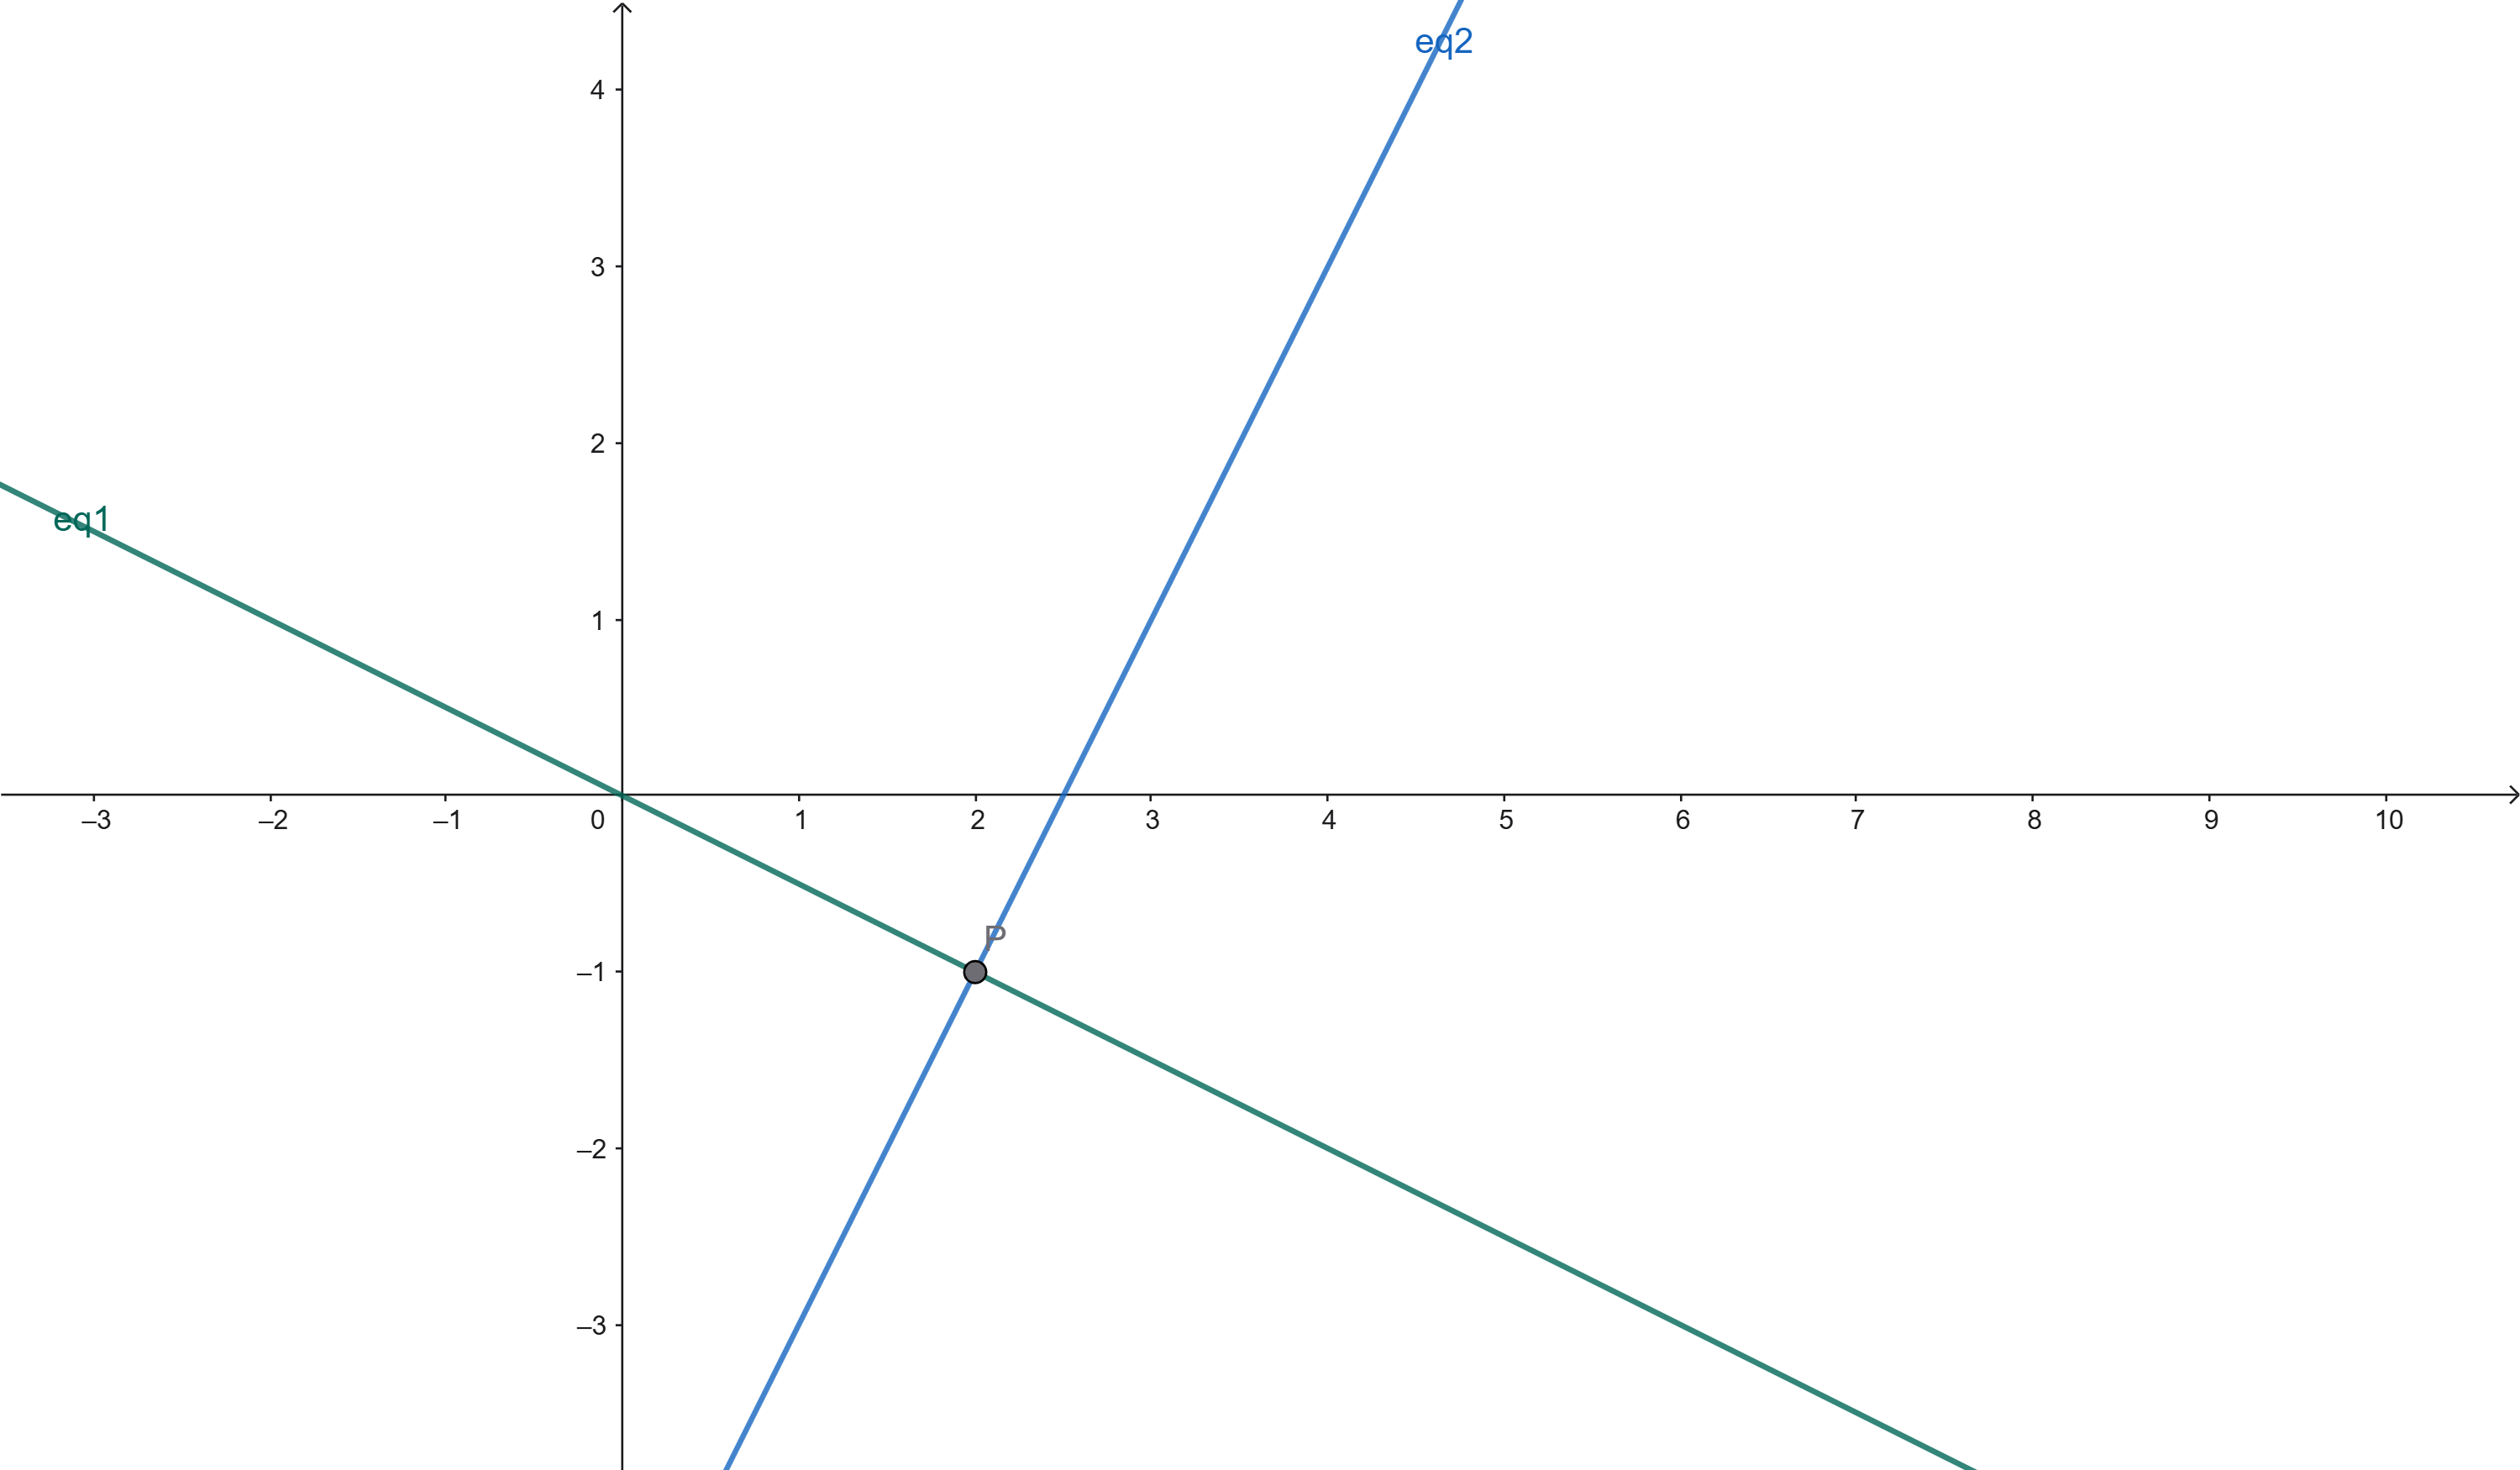
\includegraphics[width=1.0\linewidth]{imgs/alglin-01-sistema-linear}
	\caption[Exemplo de sistema linear]{exemplo de sistema linear (arquivo pessoal)}
	\label{fig:alglin-01-sistema-linear}
\end{figure}


Resolver este sistema não é uma tarefa difícil: da primeira equação, sabemos que $y = -\dfrac{x}{2}$. Da segunda equação, sabemos que $y = 2x - 5$. A solução procurada é exatamente o ponto $P$ em que as duas retas se intersectam (neste caso, $P = (2, -1)$). No entanto, esta abordagem nos revela um modo de pensar, ao qual chamaremos de \textbf{"row picture"}: estamos olhando para as linhas do sistema linear. Em uma representação geométrica, esta abordagem se preocupa com o que as equações representam geometricamente (neste caso, duas retas em $\mathbb{R}^2$ que se interceptam em um único ponto).

Por outro lado, existem uma abordagem mais interessante à qual chamaremos de \textbf{"column picture"}, na qual olharemos para o sistema linear como uma combinação linear de vetores-coluna. No entanto, nós ainda não introduzimos os conceitos de "vetor" e de "combinação linear". Nós o faremos agora de uma maneira provisória (pois, de fato, uma definição formal de vetor só poderá ser dada quando introduzirmos o conceito de espaço vetorial).

\begin{Definition}[Definição provisória de vetor]
	Um \textbf{vetor} pode ser visto como uma lista de números sobre os quais podemos fazer duas operações: soma e multiplicação por escalar.
\end{Definition}

Alguns exemplos de vetores são:

$$
\begin{bmatrix}
	3 \\ 2 \\ 4
\end{bmatrix},
\begin{bmatrix}
	0 \\ -1
\end{bmatrix},
\begin{bmatrix}
	10 \\ 5 \\ -6 \\ 7
\end{bmatrix}.
$$

Quando nós representamos os vetores como acima, tais vetores são chamados de \textbf{vetores-coluna}. De igual modo, se representarmos um vetor em uma linha (por exemplo, $\begin{bmatrix} 2 & 10 & -5 & 11 & 3 \end{bmatrix}$), nós o chamaremos de \textbf{vetor-linha}. Na maior parte do tempo, nós consideraremos que um vetor $v$ é um vetor-coluna (e que $v^T$ é um vetor-linha, mas não se preocupem com esta notação agora, no momento certo nós a introduziremos).

Pensemos em dois vetores $x$ e $y$ em $\mathbb{R}^3$, definidos por $x = \begin{bmatrix} x_1 \\ x_2 \\ x_3 \end{bmatrix}$ e $\begin{bmatrix} y_1 \\ y_2 \\ y_3 \end{bmatrix}$. Seja ainda $\alpha\in\mathbb{R}$ um escalar. Então, nós definimos a soma $x + y$ por:

$$
x + y = \begin{bmatrix}
	x_1 + y_1 \\
	x_2 + y_2 \\
	x_3 + y_3
\end{bmatrix}
$$
e a multiplicação por escalar por:

$$
\alpha x = \begin{bmatrix}
	\alpha x_1 \\
	\alpha x_2 \\
	\alpha x_3
\end{bmatrix}.
$$

\begin{Example}
	Sejam $u = \begin{bmatrix}
		3 \\
		1 
	\end{bmatrix}$ e $v = \begin{bmatrix}
	1 \\
	-1
	\end{bmatrix}$. Então, $u, v, u + v, u - v, -u, -v, 2u$ são conforme indicado na figura a seguir:
	
	\begin{figure}[H]
		\centering
		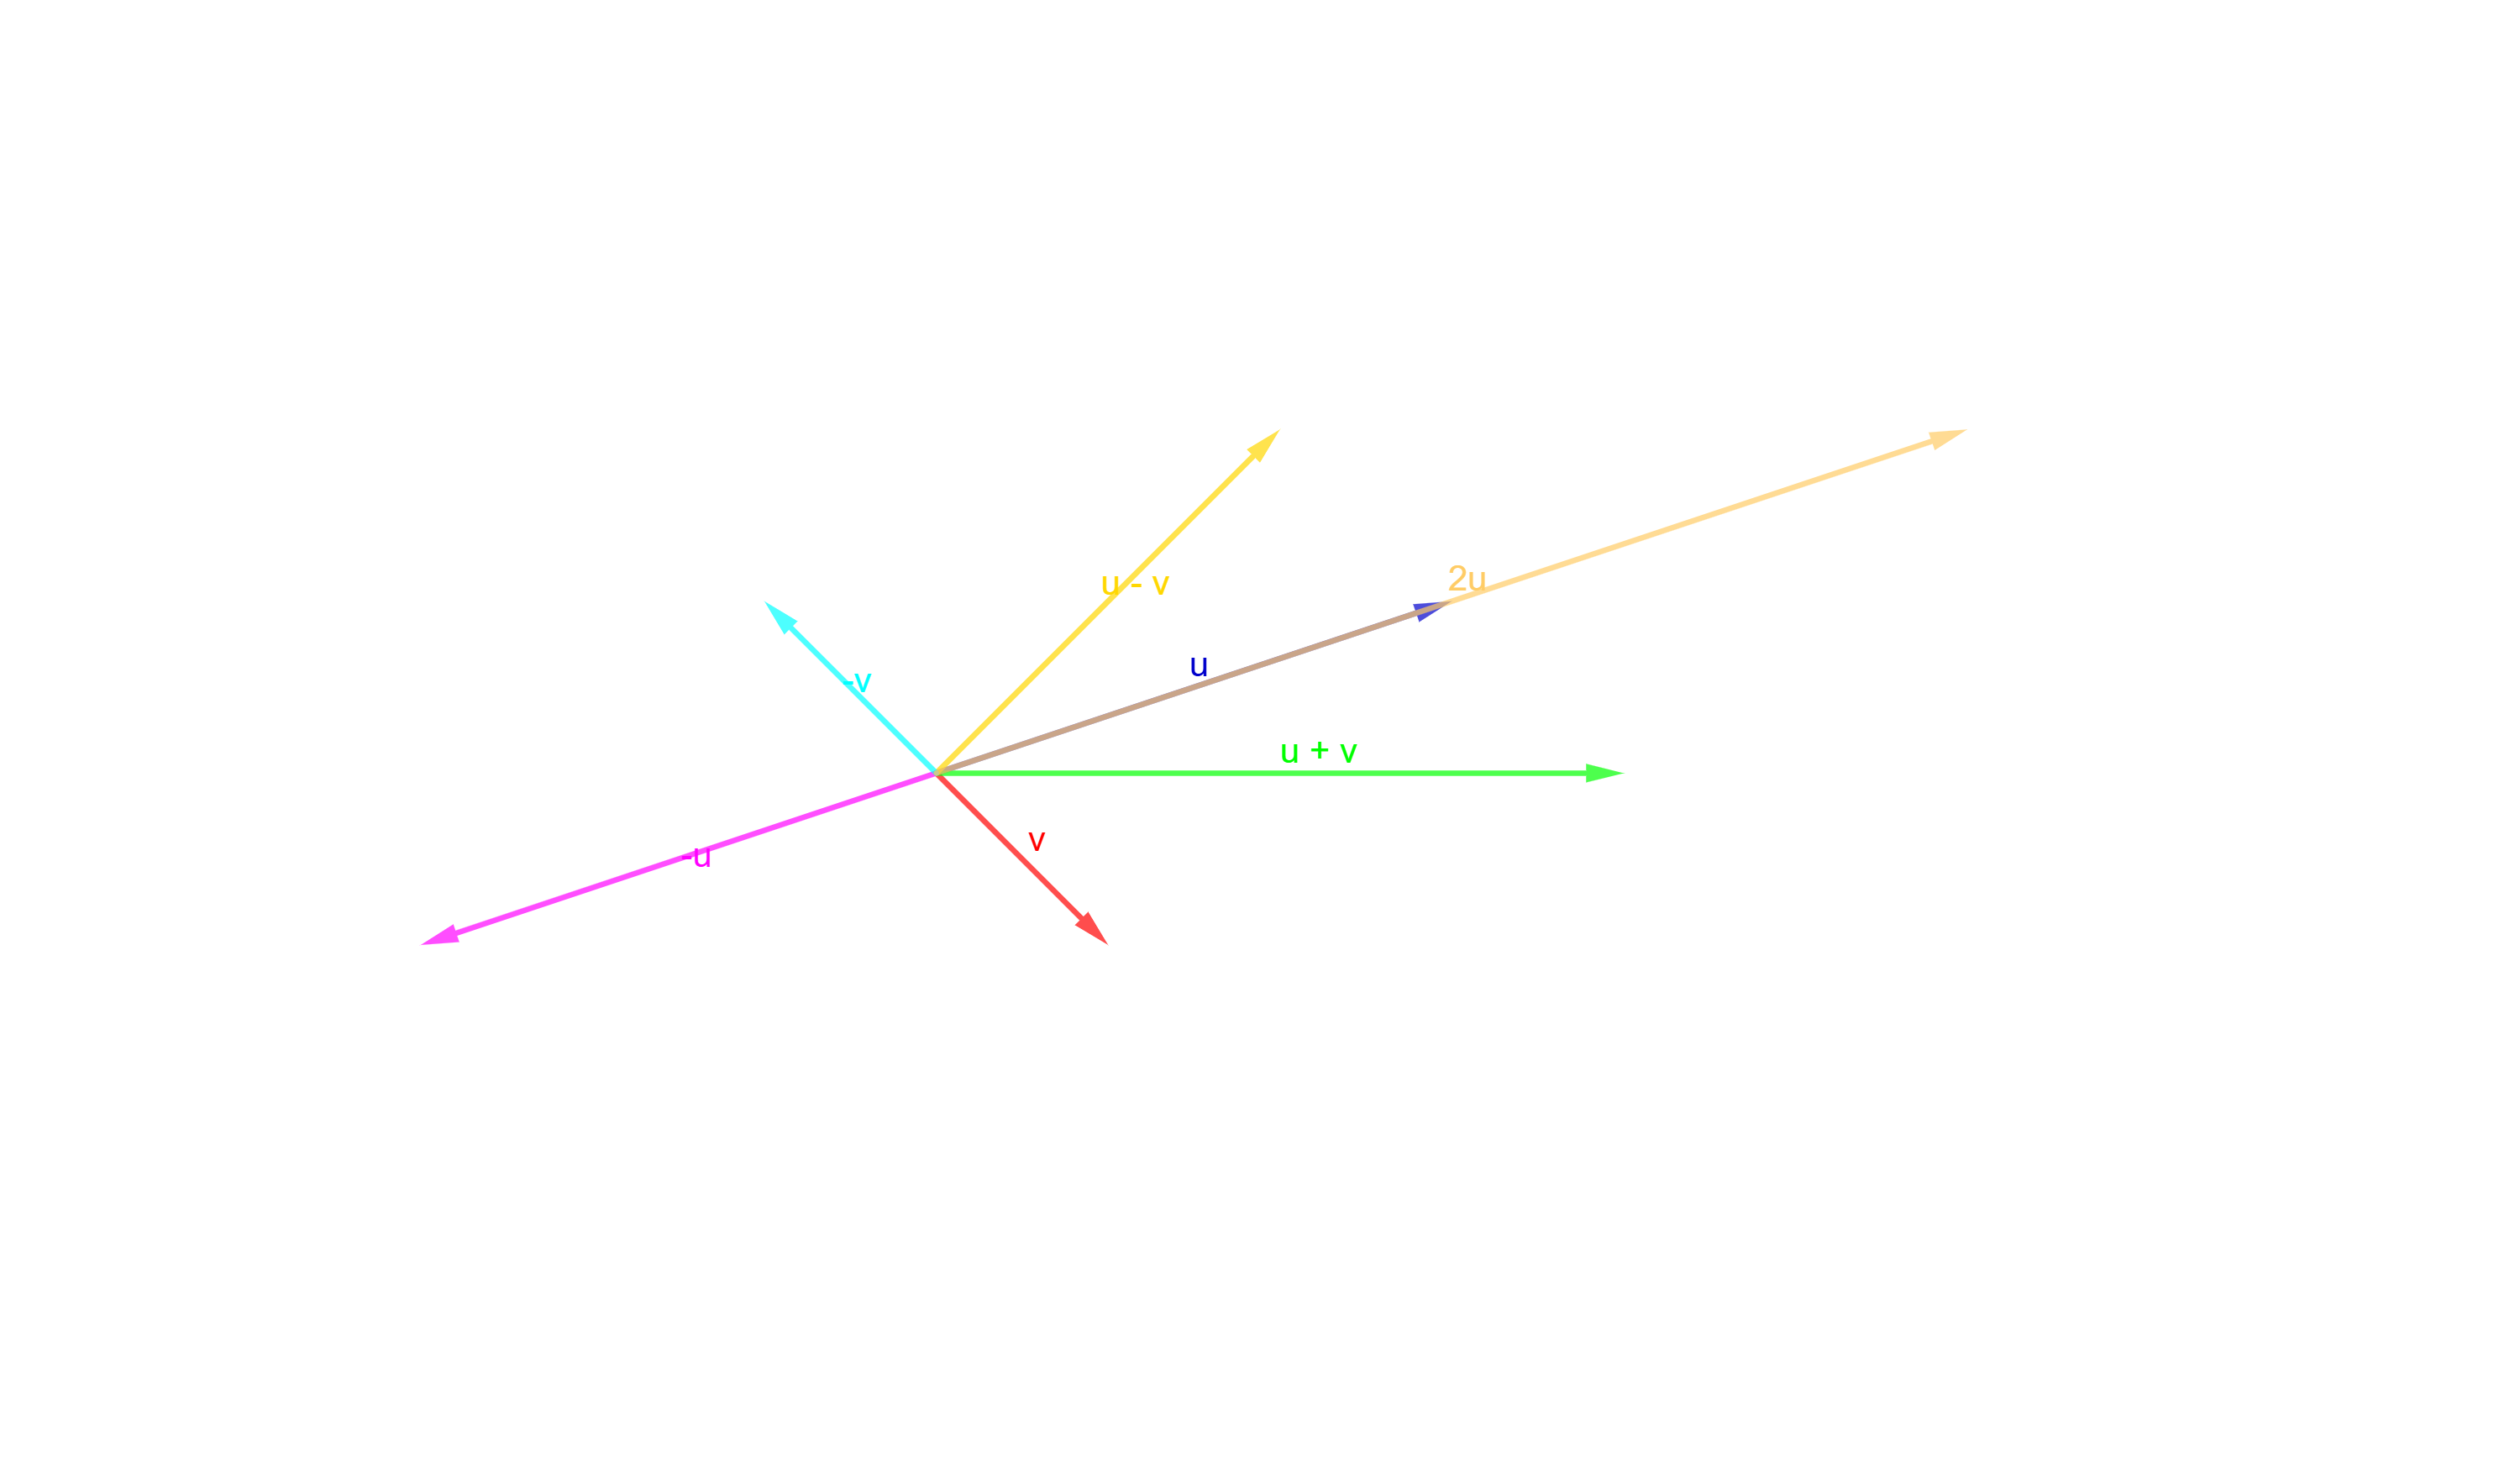
\includegraphics[width=1.0\linewidth]{imgs/alglin-02-vetores}
		\caption[Operações entre vetores]{Operações entre vetores (arquivo pessoal)}
		\label{fig:alglin-02-vetores}
	\end{figure}
	
	
\end{Example}

Por sua vez, tendo definido provisoriamente o conceito de vetor, vamos fazer uma definição para o conceito de combinação linear:

\begin{Definition}[Combinação linear]
	Sejam $v_1$, $v_2$, ... , $v_n$ vetores em um mesmo espaço, e $\alpha_1, \alpha_2, ... , \alpha_n$ escalares em $\mathbb{R}$. Uma \textbf{combinação linear} destes vetores é definida como qualquer vetor $v$ tal que
	
	$$
	v = \alpha_1v_1 + \alpha_2v_2 + \cdots + \alpha_nv_n.
	$$
\end{Definition}

Para ilustrar este conceito como um exemplo, nós podemos voltar ao sistema linear que nós vimos no começo do capítulo. Recordando, nós estamos trabalhando com o sistema

$$
\begin{cases}
	x + 2y = 0 \\
	2x - y = 5
\end{cases}.
$$

Ao invés de olhar para o sistema por uma abordagem em linha, nós podemos analisar este sistema como uma combinação linear dos vetores-coluna de coeficientes , que produz um novo vetor-coluna. Isto deve ter parecido confuso em palavras, então vamos ilustrar:

Sabemos que $x$ e $y$ são escalares, que ainda não sabemos quem são. Por outro lado, na primeira equação, $x$ é multiplicado por $1$, e na segunda equação, $x$ é multiplicado por 2. Como vimos acima, isso pode ser representado por multiplicação do escalar $x$ pelo vetor $\begin{bmatrix} 1 \\ 2 \end{bmatrix}$. Usando um raciocínio semelhante para $y$, nós obtemos a multiplicação do escalar $y$ pelo vetor $\begin{bmatrix} 2 \\ -1 \end{bmatrix}$. Olhando para o lado direito da equação, o vetor $\begin{bmatrix} 0 \\ 5 \end{bmatrix}$ pode ser escrito como uma combinação linear dos vetores $\begin{bmatrix} 1 \\ 2 \end{bmatrix}$ e $\begin{bmatrix} 2 \\ -1 \end{bmatrix}$.

Em termos matemáticos, isso é representado pela seguinte equação:

$$
x\begin{bmatrix} 1 \\ 2 \end{bmatrix} + y\begin{bmatrix} 2 \\ -1 \end{bmatrix} = \begin{bmatrix} 0 \\ 5 \end{bmatrix}.
$$

Esta é exatamente a abordagem "column picture" do sistema linear: ele pode ser visto como uma combinação linear de vetores-coluna. E, de fato, esta abordagem é mais fácil de enxergar do que a abordagem "row picture", pois não é geometricamente fácil olhar para um plano em $\mathbb{R}^6$, ou para uma reta em $\mathbb{R}^{729}$.

\section{Representação Matricial de Sistemas Lineares}

Por sua vez, há uma outra forma ainda (e a mais importante) de se representar um sistema linear qualquer. Para fazer isso, nós introduziremos o conceito de matriz:

\begin{Definition}[Matriz]
	Uma \textbf{matriz} é um conjunto de números organizado de forma retangular, ou seja, uma matriz $A$ é tal que:
	
	$$
	A = \begin{bmatrix}
		a_{11} & a_{12} & \cdots & a_{1n} \\
		a_{21} & a_{22} & \cdots & a_{2n} \\
		\vdots & \vdots & \ddots & \vdots \\
		a_{m1} & a_{m2} & \cdots & a_{mn}
	\end{bmatrix}.
	$$
\end{Definition}

Nós chamamos de $a_{ij}$ ao elemento que está na linha $i$ e na coluna $j$ da matriz.

Voltemos para o sistema linear com o qual estávamos trabalhando. Primeiramente, nós tínhamos entendido o sistema como elementos geométricos em $\mathbb{R}^2$ (row picture). Em seguida, nós entendemos o sistema como uma combinação linear de vetores-coluna (column picture). Agora, nós queremos dar um passo além e entender o sistema como a multiplicação de uma matriz por um vetor. Ou seja, queremos poder dizer que:

$$
\begin{bmatrix}
	1 & 2 \\
	2 & -1
\end{bmatrix}
\begin{bmatrix}
	x \\
	y
\end{bmatrix} = 
\begin{bmatrix}
	0 \\
	5
\end{bmatrix}.
$$

Não só isto é perfeitamente possível, como também esta é a forma como trabalharemos em muitos casos ao longo do curso (mas, de igual modo, o conceito de combinação linear será muito importante, como ainda veremos). Para realizar esta multiplicação, nós podemos pensar de duas formas: pelas linhas ou pelas colunas da matriz.

Se nós temos uma matriz $A = \begin{bmatrix}
	linha~1 \\
	linha~2 \\
	\vdots \\
	linha~m
\end{bmatrix}$ e um vetor $x$, podemos pensar que $Ax = \begin{bmatrix}
	linha~1 \cdot x \\
	linha~2 \cdot x \\
	\vdots \\
	linha~m \cdot x
\end{bmatrix}$, onde $\cdot$ indica uma operação entre vetores que definiremos em breve: o produto interno euclidiano.

Por outro lado, se ao invés de olharmos para as linhas de $A$, nós olharmos para as suas colunas, se nós definimos $A = \begin{bmatrix} coluna~1 & coluna~2 & \cdots & coluna~n \end{bmatrix}$, e $x = \begin{bmatrix}
	x_1 \\
	x_2 \\
	\vdots \\
	x_n
\end{bmatrix}$, nós temos que $Ax = x_1[coluna~1] + x_2[coluna~2] + ... + x_n[coluna~n]$. Ou seja, nós temos duas informações: $Ax$ é um vetor, e $Ax$ pode ser escrito como a combinação linear das colunas de $A$.

Olhemos novamente para o sistema linear que estávamos estudando: vamos fazer a operação que desejávamos obter para concluir que esta representação equivale ao sistema linear que nós tínhamos antes:

$$
\begin{bmatrix}
	1 & 2 \\
	2 & -1
\end{bmatrix}
\begin{bmatrix}
	x \\
	y
\end{bmatrix}
=
x\begin{bmatrix}
	1 \\
	2
\end{bmatrix}
+
y\begin{bmatrix}
	2 \\
	-1
\end{bmatrix}
=
\begin{bmatrix}
	0 \\
	5
\end{bmatrix}.
$$

Nós podemos estender o mesmo raciocínio para qualquer sistema linear de $m$ equações e $n$ incógnitas e concluir que, se $A$ é a matriz dos coeficientes do sistema, $x$ é o vetor das incógnitas e $b$ é o vetor dos termos independentes, todo sistema linear pode ser escrito como

\begin{center}
	\fbox{$Ax = b$}
\end{center}

Algo importante a se notar é que, para todas as operações que nós vamos desenvolver, as dimensões das matrizes e dos vetores devem estar corretas. No caso da multiplicação de uma matriz por um vetor, por exemplo, se $A$ é uma matriz com $m$ linhas e $n$ colunas (denotamos por $m\times n$), $x$ deve ser um vetor $n\times 1$, e a saída $b$ será um vetor $m\times 1$. Igualmente, somas de vetores só fazem sentido se as dimensões dos vetores somados forem iguais.

\section{Classificação de Sistemas Lineares}

Como é possível imaginar, nem sempre um sistema linear possuirá uma única solução. É possível que o sistema não possua nenhuma solução, e também é possível que o sistema possua infinitas soluções. Assim sendo, nós podemos classificar um sistema linear quanto à quantidade de soluções que ele possui:

\begin{itemize}
	\item \textbf{Sistema Possível e Determinado (SPD)}: possui uma única solução;
	\item \textbf{Sistema Possível e Indeterminado (SPI)}: possui infinitas soluções;
	\item \textbf{Sistema Impossível (SI)}: não possui nenhuma solução.
\end{itemize}

Vejamos alguns exemplos:

\begin{Example}[SPD]
	$$
	\begin{cases}
		x + 2y = 0 \\
		2x - y = 5
	\end{cases}
	$$
\end{Example}

\begin{Example}[SPI]
	$$
	\begin{cases}
		x + 2y = 4 \\
		2x + 4y = 8
	\end{cases}
	$$
\end{Example}

\begin{Example}[SI]
	$$
	\begin{cases}
		x + 2y = 4 \\
		2x + 4y = 7
	\end{cases}
	$$
\end{Example}

Como sugestão pessoal, pensem no significado geométrico destes três casos quando estamos lidando com sistemas lineares $2\times 2$.

\section{Produto Interno Euclidiano}

Nós vamos agora definir uma importante operação entre vetores: o produto interno euclidiano. É importante saber que o produto interno euclidiano é apenas \textbf{um} produto interno. No entanto, nós não definiremos formalmente o conceito de produto interno agora porque tal definição dependerá do conceito de espaço vetorial. Dito isso, vamos à definição:

\begin{Definition}[Produto Interno Euclidiano]
	Sejam $x$ e $y$ dois vetores $n\times 1$. O \textbf{produto interno euclidiano} é definido como:
	
	$$
	x\cdot y = \sum\limits_{i = 1}^{n} x_iy_i = x_1y_1 + x_2y_2 + \cdots + x_ny_n.
	$$
\end{Definition}

Duas propriedades importantes do produto interno euclidiano são a simetria ($x\cdot y = y\cdot x$) e a linearidade ($(\alpha x + z) \cdot y = \alpha(x\cdot y) + z\cdot y$).

% Definir melhor a linearidade
